\setcounter{chapter}{12}
\setcounter{section}{0}
\setcounter{figure}{0}
\setcounter{equation}{0}
\setcounter{table}{0}
\appendix 
\addcontentsline{toc}{chapter}{Appendix}

\chapter{A More Complicated Physical Pendulum}\label{appendix_walk}
We can make a more complicated physical pendulum by assuming the mass of the leg is linearly decreasing from the hip to the foot, i.e., the leg is more massive at the hip and less massive at the foot. See Fig.~\ref{FigA-1}
\begin{figure}[h]
	\centering
	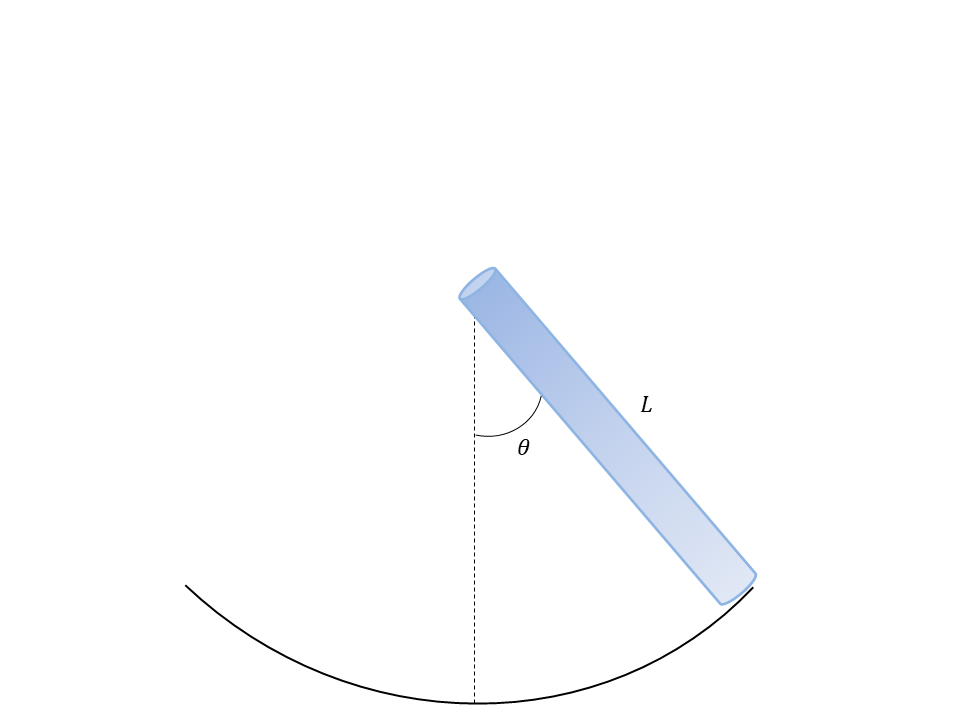
\includegraphics[width=\textwidth]{./figures/Appendix/LinearPhysPend.png}
	\caption{A physical pendulum composed of a rod with linearly-dependent mass density.}
	\label{FigA-1}
\end{figure} 
To do this we must calculate the center of mass and the moment of inertia. Fortunately, these have very similar methods of calculation. The center of mass is calculated as
\begin{equation}\label{Rcmeqn}
    R_{cm} = \frac{1}{M}\sum_i m_i x_i \rightarrow \frac{1}{M}\int_0^L dm\cdot x
\end{equation}
Before we assume the leg has a linear mass density decreasing from hip to foot, let's verify that the center of mass of the uniform cylinder is $R_{cm}=L/2$. The mass distribution looks like a constant density.
$$\lambda = \frac{dm}{dx} = \frac{M}{L}$$
where $M$ is the total mass of the leg, and $L$ is the total length of the leg. Rearranging for $dm$ gives
$$dm = \frac{M}{L} dx$$
The center of mass integral is written
\begin{align}
    R_{cm} &= \frac{1}{M}\int_0^L \frac{M}{L}x\cdot dx\nonumber\\
    R_{cm} &= \frac{1}{M}\frac{M}{L}\frac{x^2}{2}\Bigg|_0^L\nonumber\\
    R_{cm} &= \frac{1}{L}\frac{L^2}{2}\nonumber\\
    R_{cm} &= \frac{L}{2}\nonumber
\end{align}
Okay, the method seems to check out. For the improved model where the leg is a cylinder with linear mass distribution, we can write that linear density as
$$\lambda = \frac{dm}{dx} = A\left(L-x\right)$$
where $A$ is a constant similar to $M/L$ above but different (units are kg/m$^2$) for the non-uniform mass distribution. Rearranging this equation
\begin{equation}
   dm = A\left(L-x\right)dx
\end{equation}
Substituting this into Eqn.~\ref{Rcmeqn}, we get
\begin{align}\label{Rcm}
    R_{cm} &= \frac{1}{M}\int_0^L A\left(L-x\right)x\cdot dx\nonumber\\
    R_{cm} &= \frac{A}{M}\left(\frac{Lx^2}{2}-\frac{x^3}{3}\right)\Bigg|_0^L\nonumber\\
    R_{cm} &= \frac{A}{M}\frac{L^3}{6}
\end{align}

The moment of inertia is calculated similarly as
\begin{equation}\label{momInert}
    I = \sum_i m_i x_i^2 \rightarrow \int_0^L dm\cdot x^2
\end{equation}
Using our linear mass density again, we get
\begin{align}\label{momInert2}
    I &= \int_0^L A\left(L-x\right)x^2 dx\nonumber\\
    I &= A\left(\frac{Lx^3}{3}-\frac{x^4}{4}\right)\Bigg|_0^L\nonumber\\
    I &= \frac{AL^4}{12}
\end{align}

Now, we can use the step time that was derived in chapter 1 on Locomotion.
\begin{align}\label{step}
    \tau &= \pi\sqrt{\frac{I}{RMg}}\nonumber\\
    \tau &= \pi\sqrt{\frac{\frac{AL^4}{12}}{\frac{AL^3}{6M}Mg}}\nonumber\\
    \tau &= \pi\sqrt{\frac{L}{2g}}
\end{align}
We see that this step time is smaller by 25\% than the uniform cylinder because the fraction in the square root goes from $2/3$ to $1/2$.

\chapter{Fluid Friction and Viscosity}\label{appendix_fluid}

The inter-layer force proposed by Newton $$F_{visc} = \eta A \frac{dv}{dr}$$
describes the viscous (frictional) forces between two layers of fluid. If the layers are considered to be concentric cylinders sharing the central axis of the cylinder, we can write the area that two layers share as the surface area of a cylinder $ A_{cyl} = 2\pi rL$.
Next, we consider the situation where this viscous force is exactly balanced by the pressure force pushing fluid down the cylinder.
$$F_{push} = \Delta P A_{cross-section},$$
where the area is now the cross-sectional (circular face) area where the fluid is being pushed into the vessel. The change is pressure comes from the fact that a pushing force is on one end of the vessel, and no force exists on the other end. This cross-sectional area is $\pi r^2$. Starting with Newton's Second Law
$$\sum F = F_{visc}+F_{push} = 0.$$
In this equilibrium condition, velocity is constant, but as we'll see the actual value of the velocity depends on the radius at which the fluid flows down the vessel. Substituting the area and moving the push force to the right hand side, we get
$$\eta \cdot 2\pi rL\frac{dv}{dr} = - \Delta P \pi r^2.$$

Let's solve for $v$ by moving anything not involving $v$ to the right hand side.
$$dv = -\frac{\Delta P}{2\eta L} r dr$$
Next, we can get the velocity at a particular r by looking at a the integral contribution over small increments, $dr$.
$$\int dv = - \frac{\Delta P}{2\eta L} \int r dr$$
This gives
\begin{align}\label{eq-appA1}
v(r) &= -\frac{\Delta P}{2\eta L} \frac{r^2}{2} + C \nonumber\\
      &= -\frac{\Delta P}{4\eta L}r^2+C
\end{align}
We know the velocity cannot be zero at $r=0$, the center of the vessel. The velocity at the outside edge where $r=R$, the velocity is zero, and the constant $C$ is
$$C =\frac{\Delta P}{4\eta L} R^2,$$
where $R$ is the radius of the vessel. This gives the equation {eqn2-7}.
$$v(r) = \Delta P\frac{R^2-r^2}{4\eta L}$$
From this we see that the velocity is zero at the edge of the vessel and is maximum at the center. It follows a parabolic velocity profile.

%\chapter{more?}